% ==================================================
% 4. Use Cases
% ==================================================
\section{Use Cases}

% --------------------------------------------------
% 4.1 Identification of Use Cases by Actor
% --------------------------------------------------

Based on the system analysis, the main use cases for each actor are summarized below. These use cases represent high-level functional interactions with the AgriGov Market platform.

% =========================
% Buyer
% =========================
\subsection{Buyer}

The buyer is considered the end user of the platform so he will have the ability to search through the available products offered by the farmers, which will be helpful for them to purchase the required products. They will be able to place new orders or cancel their existing ones. In addition, they will have the ability to monitor their deliveries and their previous purchase history. Once they receive their ordered products, they will have the ability to provide feedback and evaluations, which will be helpful to improve the quality of the products and increase trust between buyers and farmers.

\begin{figure}[H]
	\centering
	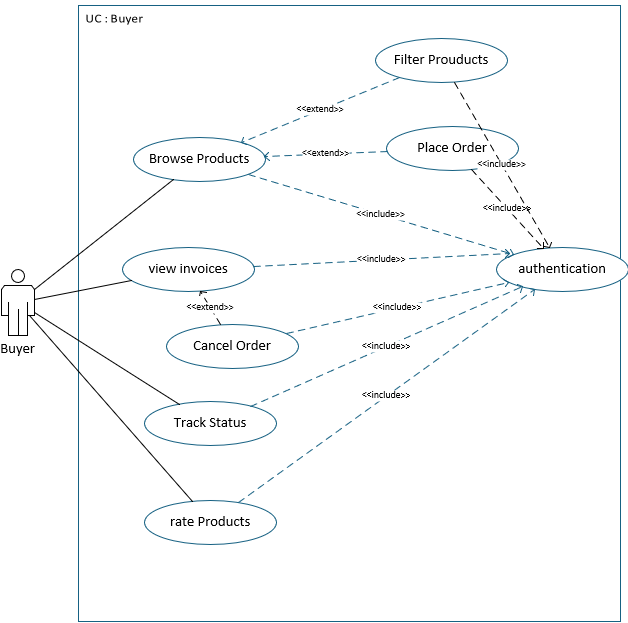
\includegraphics[width=0.95\textwidth]{images/diagrammes/buyerUCD}
	\caption{Use Case Diagram -- Buyer}
	\label{fig:buyer_ucd}
\end{figure}


% =========================
% Farmer
% =========================
\subsection{Farmer}

The farmer is  responsible for providing the agricultural products on  the platform. he has the ability to manage information of the farm and the products being offered, Moreover, the farmer has the responsibility of managing orders from customers, including processing purchase requests while keeping track of the status of each purchase order and update that status. The farmer also has access to information regarding market prices, enabling them to keep track of the latest trends in the agricultural market. Finally, the farmer has the responsibility of coordinating transportation requests, ensuring that products are transported to customers.


\begin{figure}[H]
	\centering
	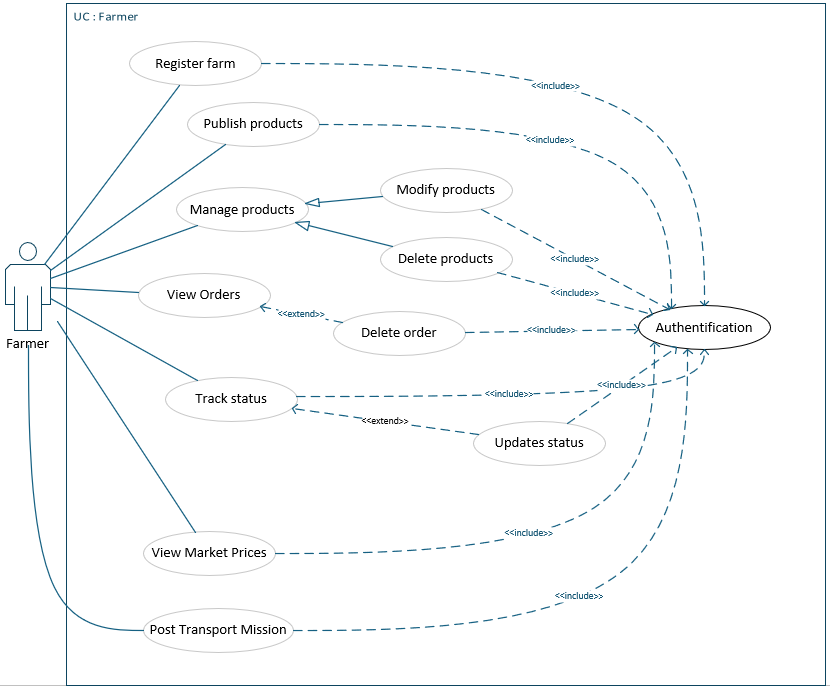
\includegraphics[width=1.05\textwidth]{images/diagrammes/farmerUCD}
	\caption{Use Case Diagram -- Farmer}
	\label{fig:farmer_ucd}
\end{figure}



% =========================
% Transporter
% =========================
\subsection{Transporter}

The function of the transporter is to handle the logistics in the delivery of the agricultural products to the buyers. Transporters are responsible for managing their transportation availability in the system, which allows them to indicate when they are available to handle the delivery request. The transporters are able to accept or reject the delivery requests submitted to transport the products. After that, the transporters are responsible for executing the delivery mission by transporting the products to the farmer or the destination. During the execution of the delivery mission, the transporters are responsible for managing the delivery status to ensure transparency in the process.


\begin{figure}[H]
	\centering
	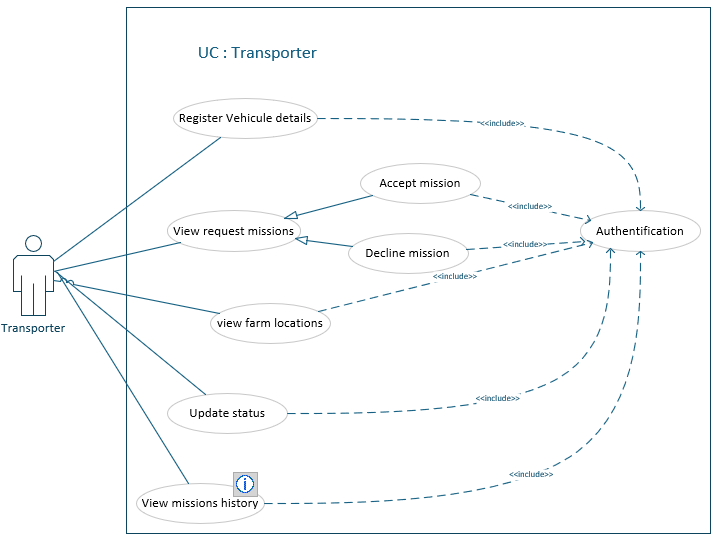
\includegraphics[width=1.05\textwidth]{images/diagrammes/transporterUCD}
	\caption{Use Case Diagram -- Transporter}
	\label{fig:transporter_ucd}
\end{figure}


% =========================
% Ministry (Administrator)
% =========================
\subsection{Ministry (Administrator)}

The ministry oversees and regulates the official information provided within the platform to ensure that the system is well governed and efficient. The ministry is also responsible for the management of the validation of the users and the regulation of access to the system, ensuring that the users are properly authorized, for instance, the farmers, the buyers, and the transporters. The ministry is also responsible for regulating the various products and the official prices within the market to ensure that there is transparency and fairness within the agricultural market. The ministry is also responsible for overseeing the overall operations within the system, including the activities within the market, to ensure that the activities within the system are in conformity with the regulations and standards.

\begin{figure}[H]
	\centering
	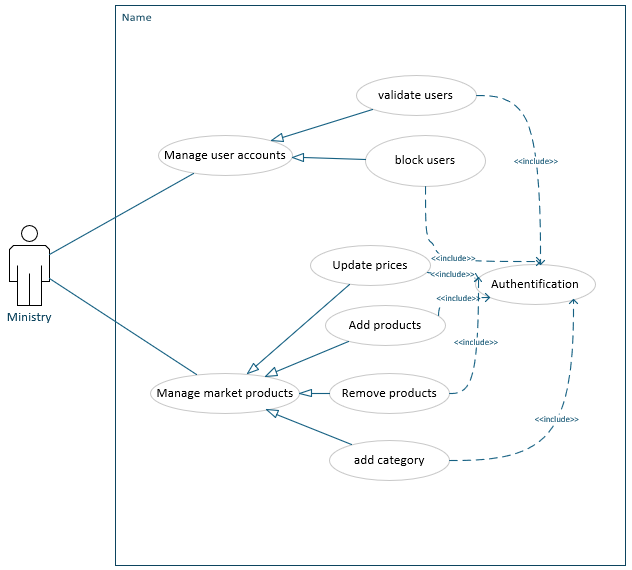
\includegraphics[width=0.95\textwidth]{images/diagrammes/ministryUCD}
	\caption{Use Case Diagram -- Ministry (Administrator)}
	\label{fig:ministry_ucd}
\end{figure}
we resume the use-cases in the globaleUCD below :
%----------global-UC------
\begin{figure}[H]
	\centering
	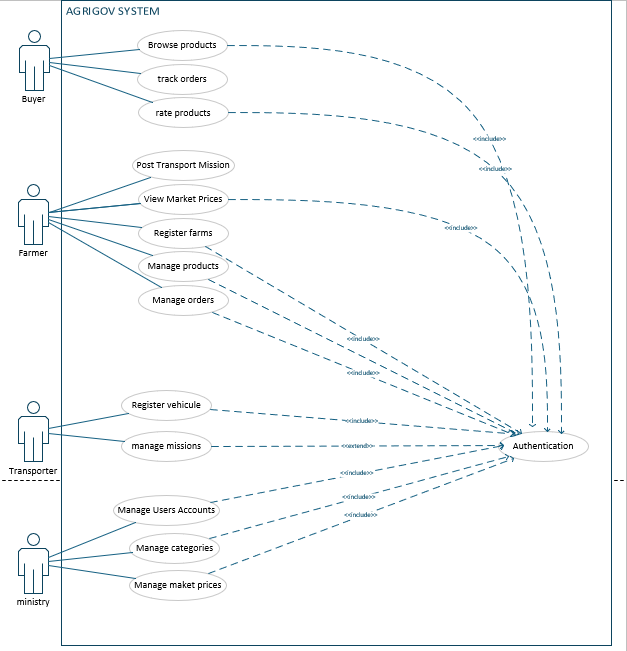
\includegraphics[width=1.15\textwidth]{images/diagrammes/GlobalUCD}
	\caption{Use Case Diagram -- Globale}
	\label{fig:Global_UC}
\end{figure}